% CVPR Supplementary Material; see https://github.com/cvpr-org/author-kit
\documentclass[10pt,twocolumn,letterpaper]{article}
\usepackage[review]{cvpr}
%% This file contains a number of tweaks that are typically applied to the main document.
%% They are not enabled by default, but can be enabled by uncommenting the relevant lines.


%%
%% Official support for 2-column teaser figure
%%
\usepackage{cuted} %< for strip environment

%%
%% For auto-referencing of figures (see fig/teaser.tex and \label{} therein) 
%%
\usepackage{currfile} %< for \currfilebase macro

%%
%% caption and (global) spacing overrides
%%
\usepackage{caption} %< for "\captionof" commands (teaser)
% \setlength{\abovecaptionskip}{.5em} % space above caption
% \setlength{\belowcaptionskip}{1em} % space below caption

%%
%% Inline annotations; for predefined colors, refer to "dvipsnames" in the xcolor package:
%% https://tinyurl.com/overleaf-colors
%%
\newcommand{\red}[1]{{\color{red}#1}}
\newcommand{\todo}[1]{{\color{red}#1}}
\newcommand{\TODO}[1]{\textbf{\color{red}[TODO: #1]}}
%%
%% Disable for camera ready / submission by uncommenting these lines:
%%
% \renewcommand{\TODO}[1]{}
% \renewcommand{\todo}[1]{#1}

%%
%% Work harder in optimizing text layout. Typically shrinks text by 1/6 of page, enable
%% it at the very end of the writing process, when you are just above the page limit.
%%
% \usepackage{microtype}

%%
%% Fine-tune paragraph spacing.
%%
% \renewcommand{\paragraph}[1]{\vspace{.5em}\noindent\textbf{#1.}}

%%
%% Globally adjusts space between figure and caption.
%%
% \setlength{\abovecaptionskip}{.5em}

%%
%% Allows "the use of \paper to refer to the project name"
%% with automatic management of space at the end of the word.
%%
% \usepackage{xspace}
% \newcommand{\paper}{ProjectName\xspace}

%%
%% Commonly used math definitions.
%%
% \DeclareMathOperator*{\argmin}{arg\,min}
% \DeclareMathOperator*{\argmax}{arg\,max}

%%
%% Tighten underline.
%%
% \usepackage{soul}
% \setuldepth{foobar}

%%
%% Reconfigure paragraph (tweaks spacing)
%%

\usepackage{multirow}
\usepackage{amsfonts}
\usepackage{xr-hyper}
\externaldocument[M-]{main}
\definecolor{cvprblue}{rgb}{0.21,0.49,0.74}
\usepackage[pagebackref,breaklinks,colorlinks,allcolors=cvprblue]{hyperref}

\def\paperID{*****} % *** Enter the Paper ID here
\def\confName{CVPR}
\def\confYear{2027}

\newcommand{\bridge}{\textsc{Bridge}}
\newcommand{\medforge}{\textsc{MedForge}}
\newcommand{\medforgepp}{\textsc{MedForge++}}

\renewcommand{\thesection}{S\arabic{section}}
\renewcommand{\thetable}{S\arabic{table}}
\renewcommand{\thefigure}{S\arabic{figure}}
\renewcommand{\theequation}{S\arabic{equation}}

\title{MedForge++: Bridging Reinforcement Learning for Generalizable\\Medical Forgery Detection Across Organ Domains}
\author{Anonymous CVPR submission}

\begin{document}
\setcounter{page}{1}
\maketitlesupplementary

This supplement collects extended background that supports the main paper's Introduction and Related Work, and a per-subset breakdown of the \medforgepp{} results. Sections, tables, figures, and equations numbered with an ``S'' prefix refer to this supplement; all other references point to the main paper.

\section{Extended Background}

This section expands the background summarized in the main paper's Introduction and Related Work. It is provided for completeness and is not required to follow the main results.

\subsection{Why medical forgery detection differs from natural-image deepfake detection}
Face-swap and full-scene deepfake detectors typically exploit identity inconsistency, blending artifacts around a face, or generator-specific frequency signatures \cite{natural_deepfake_survey_2024, frequency_artifact_detection_2024}. A medical forgery, in contrast, is often a small regional edit inside an already noisy, low-contrast, modality-specific image, with no face and no identity to check \cite{medforge2026}. The forensic cues are organ-specific. A boundary artifact around an implanted kidney tumor looks nothing like an over-smoothed region left behind by a removed skin lesion, and both look nothing like the compression and sensor noise natural-image detectors are tuned to. Detectors built for natural images therefore transfer poorly to this domain, which is part of why medical forgery detection has developed as its own line of work \cite{biotampernet2026}.

\subsection{From black-box classifiers to reasoning detectors}
Early efforts targeted GAN-based tampering in CT volumes, using cascaded patch-level localization followed by texture-based classification to catch injected lung nodules \cite{ctgan2022}. As diffusion models replaced GANs for medical synthesis, detection work generally fell into two families: black-box binary classifiers that output only a verdict, and reasoning-based detectors that try to explain the verdict \cite{medical_forgery_survey_2023}. Black-box classifiers can reach high accuracy in-distribution, but clinicians are reluctant to trust a bare label with no supporting evidence, especially when it may override a radiologist's own reading \cite{explainable_medical_ai_2025, clinical_trust_ai_2024}. This has motivated a shift toward vision-language models that localize a suspicious region before producing a verdict, since a bounding box or heatmap gives a human reviewer something concrete to check \cite{medforge2026, vigil2026}.

\subsection{Reinforcement learning for forgery-aware reasoning}
Multimodal large language models are a natural fit for the reason-then-verdict paradigm, since they can be prompted to describe an image, ask diagnostic questions, and only then commit to an answer \cite{qwenvl2024, qwen3vl2025}. Reinforcement learning has emerged as the preferred way to align these models beyond supervised imitation, since a reward can directly encode what a good explanation looks like rather than relying only on a single labeled trajectory \cite{ppo2017, grpo2024}. Group-relative methods such as GRPO and its sequence-level variant GSPO remove the need for a learned value function by normalizing reward within a sampled group of completions, and have been used to align forgery-aware reasoning models including \medforge{}-Reasoner \cite{grpo2024, gspo2025}. A separate line of work argues that models are often asked to explain artifacts their vision encoder has not actually perceived, and proposes strengthening perception before reasoning is layered on top \cite{seeingbeforereasoning2025}. A growing body of work on reinforcement learning with verifiable rewards also documents that policies readily learn to game an imperfect or under-constrained reward rather than solve the intended task \cite{rewardhacking2026}, a risk that is easy to overlook when a reward stack simply sums independent terms for verdict, localization, and format.

\subsection{Cross-domain and cross-organ generalization}
Domain shift between imaging sites, scanners, and patient populations is a long-standing problem in medical imaging, and is generally worse than the equivalent shift in natural images because acquisition physics, contrast agents, and reconstruction settings vary by institution \cite{medical_domain_shift_2024, ood_generalization_survey_2024}. Cross-generator gaps have also been documented for natural-image forgery detectors, where a detector trained against one generator's artifacts degrades sharply against another, and recent work attributes much of this gap to entangled semantic and artifact information inside a shared backbone \cite{fmsd2026}. Benchmark diversity is repeatedly identified as a bottleneck: most forgery detection benchmarks, medical or natural, cover a narrow set of generators, organs, or scenes, which makes it difficult to tell whether a reported gain reflects a genuinely better method or a better fit to a narrow distribution \cite{benchmark_diversity_2025, medical_benchmark_survey_2026}. Concurrent work on biomedical figure tampering, distinct from clinical imaging, finds that forensic models trained on natural images generalize poorly to this domain, reinforcing that generalization failures in this space are the rule rather than the exception \cite{biotampernet2026}.

\section{\medforgepp{} Addition: Composition and Results by Subset}
Table~\ref{tab:pfp-subsets} gives the full composition of the \medforgepp{} addition (main paper, Section~\ref{M-sec:composition}) by individual subset. Table~\ref{tab:pfp-subsets-results} then refines the class-level \medforgepp{} results (main paper, Table~\ref{M-tab:bridge-medforgepp}) down to these same eight subsets, using the same dedicated-SFT model $W_{\mathrm{SFT}}$.

\begin{table}[h]
\centering
\small
\caption{\medforgepp{} addition, by subset.}
\label{tab:pfp-subsets}
\begin{tabular}{lrcl}
\toprule
Subset & $n$ & Mask & Label \\
\midrule
kidney\_normal & 1{,}000 & -- & real \\
kidney\_real\_tumor & 1{,}000 & \checkmark & real \\
kidney\_removal & 1{,}000 & \checkmark & deepfake \\
polyp\_normal & 800 & -- & real \\
polyp\_real & 1{,}000 & \checkmark & real \\
polyp\_removal & 1{,}000 & \checkmark & deepfake \\
kidney\_implant (FLUX) & $\sim$1{,}000 & \checkmark & deepfake \\
colon\_implant (FLUX) & $\sim$1{,}000 & \checkmark & deepfake \\
\bottomrule
\end{tabular}
\end{table} The Remove class's aggregate failure is not uniform across organs: \texttt{kidney\_removal} is a near-total failure (3.00\% accuracy, worse than always guessing ``real''), while \texttt{polyp\_removal} retains a majority of its signal (75.00\%). Implant subsets, in contrast, are uniformly strong (99--100\%) regardless of organ. This asymmetry suggests the Remove-class failure mode is driven disproportionately by kidney CT specifically, rather than being an equally weighted property of the Remove manipulation type across all organs, and is a natural target for the organ-specific failure-targeted replay we identify as future work.

\begin{table}[h]
\centering
\small
\caption{\bridge{} (dedicated \medforgepp{} SFT) accuracy by subset, $n{=}100$ each. Real-type subsets report accuracy as the fraction correctly called real; Implant/Remove subsets report the fraction correctly called deepfake.}
\label{tab:pfp-subsets-results}
\begin{tabular}{llr}
\toprule
Organ & Subset & Acc.\ (\%) \\
\midrule
\multirow{4}{*}{Kidney} & kidney\_normal (real) & 98.00 \\
 & kidney\_real\_tumor (real) & 95.00 \\
 & kidney\_implant & 100.00 \\
 & kidney\_removal & \textbf{3.00} \\
\midrule
\multirow{4}{*}{Colon} & polyp\_normal (real) & 100.00 \\
 & polyp\_real (real) & 88.00 \\
 & colon\_implant & 99.00 \\
 & polyp\_removal & 75.00 \\
\bottomrule
\end{tabular}
\end{table}

\begin{table}[h]
\centering
\small
\begin{tabular}{llrrrr}
\toprule
Method & Organ & Real & Implant & Remove & Avg \\
\midrule
\multicolumn{6}{l}{\textit{Published baselines (SIDA, FakeVLM, AIGI-Holmes, MLLMs)}} \\
\quad any & all five & -- & -- & -- & -- \\
\midrule
\multicolumn{6}{l}{\medforge{}-Reasoner (fair re-eval)} \\
 & Chest X-ray$^\dagger$ & 100.00 & 100.00 & 100.00 & 100.00 \\
 & Brain MRI$^\dagger$ & 98.80 & 100.00 & 99.71 & 99.50 \\
 & Fundus$^\dagger$ & 100.00 & 100.00 & 100.00 & 100.00 \\
 & Kidney CT & 100.00 & 27.00 & 0.00 & 56.75 \\
 & Colon Polyp & 0.50 & 100.00 & 92.00 & 48.25 \\
\midrule
\multicolumn{6}{l}{\textbf{\bridge{} (ours)}} \\
 & Chest X-ray & 96.14 & 98.67 & 97.99 & 97.64 \\
 & Brain MRI & 92.77 & 93.03 & 99.42 & 95.13 \\
 & Fundus & 96.62 & 99.66 & 98.38 & 98.17 \\
 & Kidney CT & 96.50 & 100.00 & 3.00 & 74.00 \\
 & Colon Polyp & 94.00 & 99.00 & 75.00 & 90.50 \\
\bottomrule
\end{tabular}
\caption{Per-organ, per-class accuracy (\%) across all five \medforgepp{} organs, in the same Real/Implant/Remove structure as the main paper's Table~\ref{M-tab:published-full}, computed by decomposing each model's saved per-image predictions by organ (pooled values reproduce the aggregate results in the main paper). $\dagger$: for \medforge{}-Reasoner, the three \medforge{}-90K organs are \emph{in-domain} (part of its training distribution), so those near-perfect scores are an upper bound and are not directly comparable to \bridge{}'s Cross-Forgery numbers on the same organs; the informative comparison is on the two \emph{unseen} organs, where the released \medforge{}-Reasoner collapses (Kidney~CT 56.75, Colon~Polyp 48.25) while \bridge{}, trained on \medforgepp{}, retains 74.00 / 90.50. \bridge{}'s \medforge{}-organ rows use the deployed Cross-Forgery model ($\alpha{=}0.15$); its Kidney/Colon rows use the dedicated \medforgepp{} SFT (subsets of Table~\ref{tab:pfp-subsets-results}, $n{=}100$ each), with Avg image-weighted over all four subsets. Published baselines report only pooled results, marked ``--''.}
\label{tab:per-organ-five}
\end{table}

\section{Supplementary Experiments}

\subsection{Compute Resources}
All training and evaluation was run on single NVIDIA H100 80GB HBM3 GPUs (no multi-GPU or multi-node parallelism), on a Red Hat Enterprise Linux 9.4 host with NVIDIA driver 580.126.16. The software stack was Python 3.10.13, PyTorch 2.5.1 (CUDA 12.4 build), Hugging Face Transformers 5.8.1, PEFT 0.19.1, and TRL 0.16.1. Every \bridge{} model is a rank-32 LoRA adapter (main paper, Section~\ref{M-sec:method}) on a frozen Qwen3-VL-8B-Instruct backbone, trained with batch size 1 and gradient accumulation 8. Stage-1 SFT and its failure-targeted replay continuation each run for 1 epoch over their respective training pools (tens of thousands to just over 100{,}000 records depending on regime); Stage-2 GRPO samples $G{=}8$ rollouts per prompt over a few hundred optimizer steps (Table~\ref{tab:ablation-rl}); Stage-3 interpolation applies the weight-blend equation from Section~\ref{M-sec:stage3} of the main paper directly to saved adapter weights and requires no GPU time. A single SFT training run on this hardware takes on the order of several GPU-hours to low tens of GPU-hours, scaling with training-pool size.

\subsection{Stage Contribution Ablation}
Table~\ref{tab:ablation-stage-contribution} isolates the contribution of each stage on the Cross-Forgery test set, using the model that results from adding one stage at a time: Stage 1 alone, Stage 1 with failure-targeted replay, adding Stage 2 (GRPO), and adding Stage 3 (interpolation, the interpolated model). Failure-targeted replay is the single largest driver of classification accuracy (+1.54 points over Stage 1 alone), consistent with it being the strongest classifier among our models, reported in Section~\ref{M-sec:ablation} of the main paper. GRPO trades some of that accuracy for a large localization gain (mIoU rises from 24.06 to 27.50), and interpolation recovers accuracy beyond either endpoint while retaining part of the localization gain, which is the complementary-errors mechanism analyzed in Section~\ref{M-sec:stage3} and Section~\ref{M-sec:ablation} of the main paper. Precision and recall are reported for the binary real/deepfake verdict; macro-F1 in this table uses the same binary convention rather than the main paper's per-class one-vs-rest convention (main paper, Table~\ref{M-tab:main}), so the two are not directly comparable numerically, though the relative ordering across stages is consistent either way.

\begin{table}[t]
\centering
\small
\caption{Stage contribution ablation, Cross-Forgery test set ($n{=}2{,}994$). Each row adds one stage of the \bridge{} recipe.}
\label{tab:ablation-stage-contribution}
\resizebox{\columnwidth}{!}{%
\begin{tabular}{lrrrrrr}
\toprule
Model & Acc. & F1 & Prec. & Rec. & mIoU & Loc.\ Acc. \\
\midrule
A: Stage 1 only & 94.22 & 93.71 & 92.63 & 95.37 & 22.16 & 17.75 \\
B: +Failure-Targeted Replay & 95.76 & 95.13 & 96.12 & 94.29 & 24.06 & 20.00 \\
C: +GRPO (Stage 2) & 95.26 & 94.52 & 95.82 & 93.49 & 27.50 & 22.80 \\
D: +Interpolation (BRIDGE) & 96.76 & 96.33 & 96.52 & 96.16 & 24.10 & 19.55 \\
\bottomrule
\end{tabular}%
}
\end{table}

\subsection{Fair Evaluation of the Released \medforge{}-Reasoner}
We downloaded the publicly released \medforge{}-Reasoner weights (Apache-2.0) and evaluated them with our harness. An initial run, using our own prompt template and a 448-token generation budget, produced an apparent near-total collapse (50\% accuracy, 100\% fake-recall) on both its own test set and ours. Inspection of the raw generations showed this was an artifact of our evaluation, not the model: our verdict parser matched the substring ``is a deepfake'' anywhere in the output, including inside the model's own boilerplate reasoning opener (``I am starting to analyze whether this image is a deepfake:''), which precedes its actual conclusion regardless of the true answer. We corrected the parser to search only the text following the model's final \texttt{</think>} tag (verified to be a no-op for every \bridge{}-trained model, whose templates never mention the opposite verdict before the true one) and re-ran evaluation using \medforge{}-Reasoner's own documented prompt and generation budget (2048 tokens) from its model card. We report the corrected numbers throughout the main paper; we note this detail because evaluation-harness artifacts of exactly this kind are an underappreciated risk when benchmarking externally-sourced instruction-tuned models.

\subsection{Qualitative Example}
Figure~\ref{fig:qualitative} walks through one held-out example end to end (main paper, Section~\ref{M-sec:reasoning}), from the input image through the model's step-by-step reasoning to its localized verdict.

\begin{figure}[h]
\centering
\IfFileExists{figures/qualitative_eg.png}
  {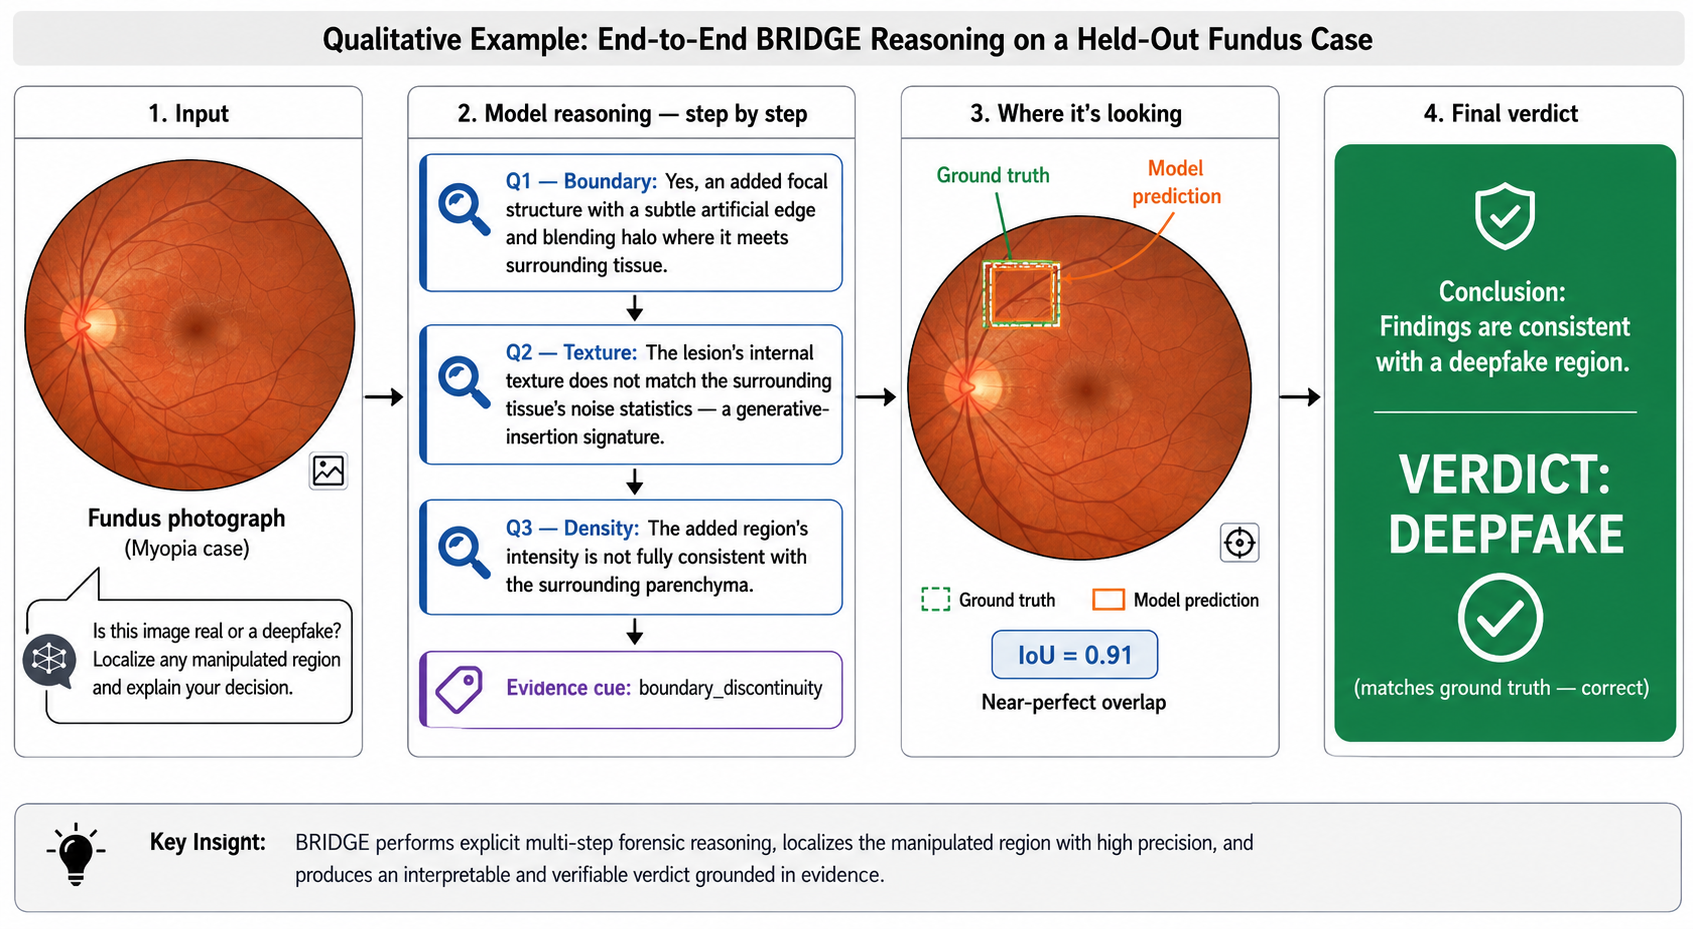
\includegraphics[width=\columnwidth]{figures/qualitative_eg.png}}
  {\fbox{\parbox{0.9\columnwidth}{\centering\vspace{2cm}[figures/qualitative\_eg.png not uploaded]\vspace{2cm}}}}
\caption{Qualitative example of \bridge{}'s end-to-end reasoning on a held-out fundus photograph (implant forgery, not seen during training). Given the image and prompt, the model answers three diagnostic questions, names an evidence cue, localizes the manipulated region (IoU~$=0.91$ against the ground-truth box), and reaches the correct verdict.}
\label{fig:qualitative}
\end{figure}

The detailed per-class comparison against every published baseline (SIDA, FakeVLM, AIGI-Holmes, generic MLLMs, \medforge{}-Reasoner) is now reported directly in the main paper (Section~\ref{M-sec:perclass}, Table~\ref{M-tab:published-full}).

\subsection{\bridge{} Per-Class Results on \medforge{}-90K}
Table~\ref{tab:bridge-medforge} reports \bridge{}'s per-class results on \medforge{}-90K in the same class/regime structure as the main paper's Table~\ref{M-tab:published-full}, with all three regimes now fully resolved across all three \bridge{} stages. Cross-Forgery and In-Domain both use the $\alpha{=}0.15$ interpolation (Stage 3), the best of the three stages in each case; Cross-Model uses the Stage-2 GRPO model $W_{\mathrm{RL}}$ directly, which we found outperforms both the Stage-1 replay-SFT endpoint and the interpolated model for this regime (Section~\ref{M-sec:ablation} of the main paper).

\begin{table}[h]
\centering
\small
\resizebox{\columnwidth}{!}{%
\begin{tabular}{lcccc}
\toprule
Class & In-Domain & Cross-Forgery & Cross-Model & Avg \\
\midrule
\multicolumn{5}{c}{\textit{Accuracy (\%)}} \\
\midrule
Real & 98.99 & 95.17 & 99.40 & 97.85 \\
Implant & 99.60 & 97.10 & 91.90 & 96.20 \\
Remove & 98.50 & 98.60 & 91.80 & 96.30 \\
\midrule
\textbf{Average} & \textbf{99.03} & \textbf{96.96} & \textbf{94.66} & \textbf{96.88} \\
\midrule
\multicolumn{5}{c}{\textit{F1 Score (\%)}} \\
\midrule
Real & 98.55 & 95.41 & 92.12 & 95.36 \\
Implant & 99.30 & 96.19 & 95.48 & 96.99 \\
Remove & 98.75 & 96.95 & 95.43 & 97.04 \\
\midrule
\textbf{Average} & \textbf{98.87} & \textbf{96.18} & \textbf{94.62} & \textbf{96.56} \\
\bottomrule
\end{tabular}%
}
\caption{\bridge{} on \medforge{}-90K, same class/regime structure as the main paper's per-class table, with all three regimes fully resolved. Cross-Forgery and In-Domain use the $\alpha{=}0.15$ interpolation (Stage 3); Cross-Model uses the Stage-2 GRPO model $W_{\mathrm{RL}}$ directly. The Avg column is the mean across the three regimes.}
\label{tab:bridge-medforge}
\end{table}

\subsection{Stage-2 (RL) Ablations}
Table~\ref{tab:ablation-rl} summarizes every Stage-2 configuration we trained. Across reward designs, $\beta$ values, and step budgets, forgery-aware RL consistently lifts localization: every mIoU is at or above Stage 1's 24.06, with the best reaching 28.84, while classification accuracy stays anchored by the supervised replay stage. Table~\ref{tab:ablation-reward} ablates each term of the classification-dominant reward: removing $R_{\mathrm{loc}}$ causes the largest mIoU drop, removing $R_{\mathrm{evid}}$ the largest accuracy and F1 drop, and removing $R_{\mathrm{fmt}}$ falls between. No single bonus is redundant.

\begin{table}[h]
\centering
\small
\caption{Stage-2 ablation, Cross-Forgery test set. All rows use the classification-dominant reward except ``Guarded reward,'' an earlier additive reward-stack baseline (terms summed rather than gated on verdict correctness).}
\label{tab:ablation-rl}
\begin{tabular}{lrrr}
\toprule
Configuration & Acc.\ & F1 & mIoU \\
\midrule
Guarded reward (baseline ablation) & 95.32 & 94.63 & 25.10 \\
$\beta{=}0$, 400 steps & 95.26 & 94.52 & 27.50 \\
$\beta{=}0$, 800 steps & 93.89 & 92.80 & \textbf{28.84} \\
$\beta{=}0.001$, 400 steps & 92.28 & 90.76 & 26.57 \\
$\beta{=}0$, lr\,$3{\times}10^{-7}$, 600 steps & 95.12 & 94.33 & 25.78 \\
\bottomrule
\end{tabular}
\end{table}

\begin{table}[h]
\centering
\small
\caption{Reward-component ablation, Cross-Forgery test set. Each row zeroes one auxiliary bonus; the verdict gate and contradiction penalties are always active.}
\label{tab:ablation-reward}
\begin{tabular}{lrrr}
\toprule
Reward variant & Acc.\ & F1 & mIoU \\
\midrule
Full reward (all terms) & 95.26 & 94.52 & 27.50 \\
\quad $-\,R_{\mathrm{loc}}$ (localization) & 94.49 & 93.58 & 26.04 \\
\quad $-\,R_{\mathrm{evid}}$ (evidence) & 93.59 & 92.47 & 27.56 \\
\quad $-\,R_{\mathrm{fmt}}$ (format) & 94.15 & 93.16 & 26.78 \\
\bottomrule
\end{tabular}
\end{table}

\subsection{Reward Target Ablation}
Table~\ref{tab:ablation-target} compares training Stage 2 against reward targets that isolate a single competency entirely, rather than removing one term from the classification-dominant reward. \emph{Localization-only} drops the verdict term altogether, rewarding only $\mathrm{IoU}(\hat b, b)$; \emph{Explanation-only} rewards only evidence grounding and output format, with no verdict or box term. Both are contrasted with the additive \emph{Guarded reward} baseline (verdict, localization, evidence, and format terms summed rather than gated) and our classification-dominant \emph{Full reward}. Localization-only reaches the highest accuracy of all four configurations (95.46) despite carrying no classification signal whatsoever, which shows GRPO does not need an explicit verdict term to preserve the classification behavior already present in the Stage-1 model $W_{\mathrm{SFT}}$ it starts from. Its mIoU is nonetheless the lowest of the four (23.32), the opposite of what a reward tuned purely for localization would be expected to produce; we attribute this to the localization-only policy having no incentive to terminate with a well-formed, confident verdict, which destabilizes the box-emission behavior learned during Stage 1. Explanation-only reaches intermediate accuracy (94.62) purely from evidence and format shaping, with no direct classification or localization term, showing some classification signal transfers indirectly through the reasoning-quality reward. Full reward remains the best trade-off across both competencies jointly, which is why we adopt it for \bridge{}.

\begin{table}[h]
\centering
\small
\caption{Reward target ablation, Cross-Forgery test set. Localization-only and Explanation-only remove the verdict term from the reward entirely, isolating a single competency; Guarded reward sums all terms without gating; Full reward is our classification-dominant design (Eq.~\ref{M-eq:reward} in the main paper).}
\label{tab:ablation-target}
\begin{tabular}{lrrr}
\toprule
Reward target & Acc.\ & F1 & mIoU \\
\midrule
Localization-only & \textbf{95.46} & \textbf{94.97} & 23.32 \\
Guarded reward (additive) & 95.32 & 94.63 & 25.10 \\
Full reward (classification-dominant) & 95.26 & 94.52 & \textbf{27.50} \\
Explanation-only & 94.62 & 94.10 & 24.07 \\
\bottomrule
\end{tabular}
\end{table}

\subsection{Full Interpolation Ratio Sweep}
Table~\ref{tab:ablation-interp-full} extends the abbreviated sweep of the main paper's Table~\ref{M-tab:ablation-interp} to the full 0.05-step grid, $\alpha \in \{0.00, \ldots, 0.40\}$, Cross-Forgery test set. Accuracy and F1 both peak at $\alpha{=}0.15$ and decline monotonically on both sides through the range tested, while mIoU increases roughly monotonically with $\alpha$ throughout.

\begin{table}[h]
\centering
\small
\caption{Full interpolation ratio sweep (Eq.~\ref{M-eq:interp} of the main paper), Cross-Forgery test set. $\alpha{=}0.00$ is the pure replay-SFT endpoint.}
\label{tab:ablation-interp-full}
\begin{tabular}{lrrr}
\toprule
$\alpha$ & Acc.\ & F1 & mIoU \\
\midrule
0.00 & 95.76 & 94.16 & 24.06 \\
0.05 & 96.33 & 95.17 & 24.13 \\
0.10 & 96.76 & 95.86 & 24.10 \\
0.15 & \textbf{96.96} & \textbf{96.18} & 24.70 \\
0.20 & 96.63 & 95.92 & 25.11 \\
0.25 & 96.53 & 95.78 & 25.14 \\
0.30 & 96.46 & 95.69 & 25.53 \\
0.35 & 96.33 & 95.41 & 25.96 \\
0.40 & 96.19 & 95.19 & \textbf{26.29} \\
\bottomrule
\end{tabular}
\end{table}

\subsection{Regime-Transfer Ablation}
Table~\ref{tab:ablation-regime-transfer} traces the three \bridge{} stages across all three regimes at a fixed $\alpha{=}0.10$. On Cross-Forgery the stages are strictly monotone in accuracy: Stage~1 (SFT) is lowest at 94.22, Stage~2 (RL) adds a modest gain to 95.26, and Stage~3 (interpolation) is best at 96.76, with F1 following the same order. This is the clearest illustration of the complementary-errors mechanism (main paper, Section~\ref{M-sec:stage3}): RL relocates part of the model's competence toward localization (mIoU rises from 22.16 to 27.50), and interpolation then recovers and exceeds the classification accuracy of either endpoint. The In-Domain and Cross-Model rows in the top block use an earlier model trained \emph{before} failure-targeted replay; there RL trades a little accuracy for mIoU and interpolation lands between the endpoints. The bottom block reports the final post-replay models at $\alpha{=}0.15$ for these two regimes: on In-Domain the monotone pattern is restored and interpolation again becomes the best of the three stages (99.03/98.91), while on Cross-Model Stage~2 (RL) remains best even at $\alpha{=}0.15$ (94.66/94.18 vs.\ interpolation's 94.36/93.86), confirming that interpolation does not help this regime regardless of the mixing ratio.

\begin{table}[h]
\centering
\small
\caption{Stage-by-stage comparison, test $n{=}2{,}994$. \emph{Top block}: pre-replay models at $\alpha{=}0.10$; on Cross-Forgery, accuracy is strictly monotone and Stage~3 (interpolation) is best. \emph{Bottom block}: the final post-replay models at $\alpha{=}0.15$ for In-Domain and Cross-Model -- on In-Domain interpolation is again best, while on Cross-Model Stage~2 (RL) remains best even at $\alpha{=}0.15$. Bold marks the best stage per regime.}
\label{tab:ablation-regime-transfer}
\begin{tabular}{llrrr}
\toprule
Regime & Stage & Acc. & F1 & mIoU \\
\midrule
\multicolumn{5}{l}{\textit{Pre-replay models, $\alpha{=}0.10$}} \\
\midrule
\multirow{3}{*}{Cross-Forgery} & Stage 1: SFT & 94.22 & 93.71 & 22.16 \\
 & Stage 2: RL & 95.26 & 94.52 & \textbf{27.50} \\
 & Stage 3: interp.\ & \textbf{96.76} & \textbf{96.33} & 24.10 \\
\midrule
\multirow{3}{*}{In-Domain} & Stage 1: SFT & \textbf{98.46} & \textbf{98.17} & 26.84 \\
 & Stage 2: RL & 98.23 & 97.89 & \textbf{28.51} \\
 & Stage 3: interp.\ & 98.40 & 98.05 & 27.47 \\
\midrule
\multirow{3}{*}{Cross-Model} & Stage 1: SFT & \textbf{93.55} & \textbf{93.44} & 24.46 \\
 & Stage 2: RL & 92.38 & 92.39 & \textbf{26.20} \\
 & Stage 3: interp.\ & 93.32 & 93.25 & 24.43 \\
\midrule
\multicolumn{5}{l}{\textit{Final post-replay models, $\alpha{=}0.15$}} \\
\midrule
\multirow{3}{*}{In-Domain} & Stage 1: SFT & 99.00 & 98.87 & 31.12 \\
 & Stage 2: RL & 98.90 & 98.76 & \textbf{33.76} \\
 & Stage 3: interp.\ & \textbf{99.03} & \textbf{98.91} & 31.54 \\
\midrule
\multirow{3}{*}{Cross-Model} & Stage 1: SFT & 94.32 & 93.83 & 28.77 \\
 & Stage 2: RL & \textbf{94.66} & \textbf{94.18} & \textbf{31.12} \\
 & Stage 3: interp.\ & 94.36 & 93.86 & 29.28 \\
\bottomrule
\end{tabular}
\end{table}

\subsection{Per-Class Error Complementarity}
Table~\ref{tab:overlap-perclass} extends the error-overlap analysis of Section~\ref{M-sec:ablation} in the main paper (Table~\ref{M-tab:overlap}) to the per-class level, breaking down agreement between the Stage-1 (replay-SFT) and Stage-2 (best RL) models on the Cross-Forgery test set by ground-truth class rather than pooling across all three. Figure~\ref{fig:ablation7-heatmap} visualizes the same breakdown. Complementarity is heavily concentrated in the Real class: $W_{\mathrm{SFT}}$ and $W_{\mathrm{RL}}$ agree on only 83.80\% of Real images, compared to 97.60\% (Implant) and 98.60\% (Remove). This means $W_{\mathrm{SFT}}$ and $W_{\mathrm{RL}}$ occasionally disagree about whether an authentic image is manipulated at all, rather than primarily disagreeing about forgery type or localization on already-flagged images. The oracle upper bound is correspondingly lower on Real (94.37\%) than on Implant (99.40\%) or Remove (99.20\%), so most of the achievable interpolation headroom identified in the main paper's Table~\ref{M-tab:overlap} lives specifically in classifying authentic images correctly.

\begin{table}[h]
\centering
\small
\caption{Per-class breakdown of Stage-1 (replay-SFT) vs.\ Stage-2 (best RL) verdict agreement, Cross-Forgery test set, extending the pooled analysis of Table~\ref{M-tab:overlap} in the main paper.}
\label{tab:overlap-perclass}
\begin{tabular}{lrrrrr}
\toprule
Class & Both OK & SFT-only & RL-only & Both wrong & Oracle \\
\midrule
Real & 83.80 & 6.14 & 4.43 & 5.63 & 94.37 \\
Implant & 97.60 & 1.00 & 0.80 & 0.60 & 99.40 \\
Remove & 98.60 & 0.10 & 0.50 & 0.80 & 99.20 \\
\midrule
\textbf{ALL} & \textbf{93.35} & \textbf{2.40} & \textbf{1.90} & \textbf{2.34} & \textbf{97.66} \\
\bottomrule
\end{tabular}
\end{table}

\begin{figure}[h]
\centering
\IfFileExists{figures/ablation7_agreement_heatmap.png}
  {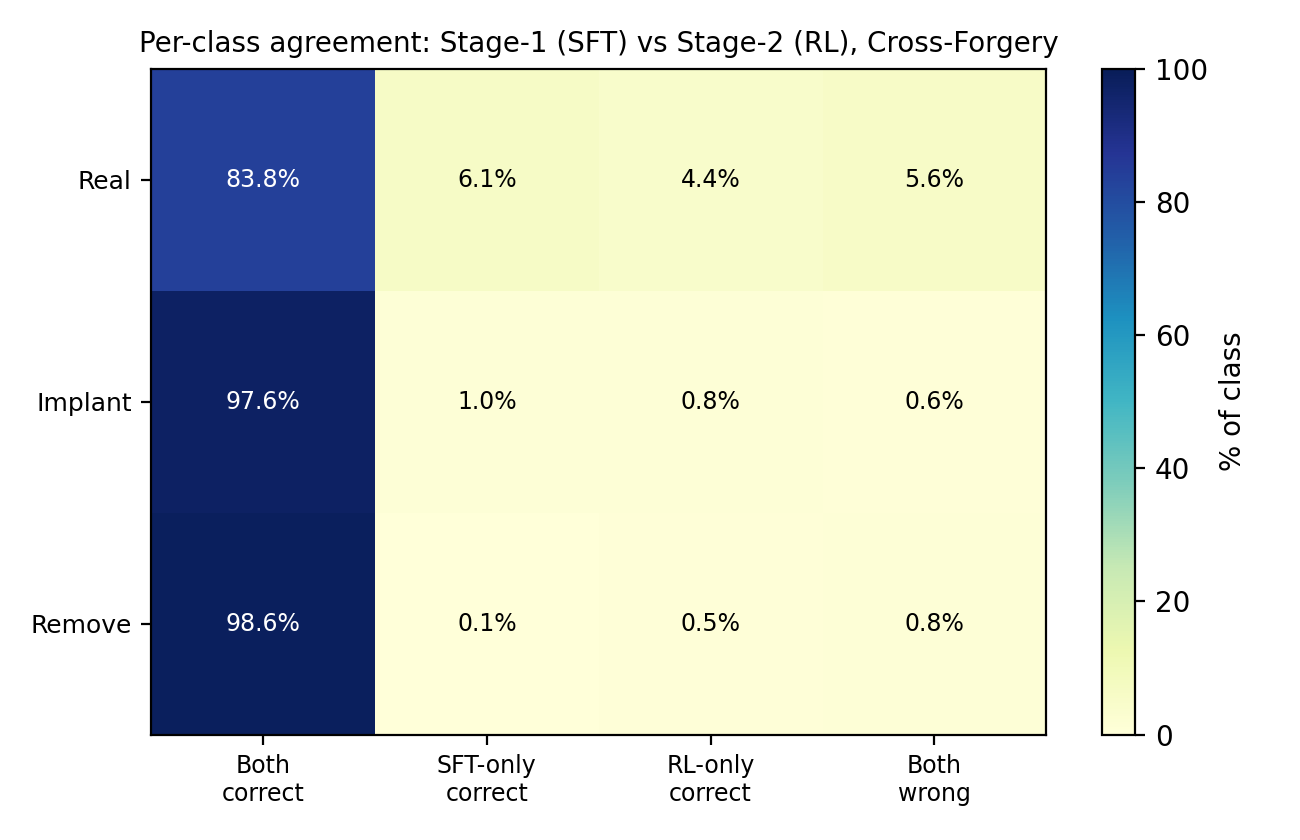
\includegraphics[width=\columnwidth]{figures/ablation7_agreement_heatmap.png}}
  {\fbox{\parbox{0.9\columnwidth}{\centering\vspace{2cm}[figures/ablation7\_agreement\_heatmap.png not uploaded]\vspace{2cm}}}}
\caption{Per-class agreement between the Stage-1 (replay-SFT) and Stage-2 (best RL) models, Cross-Forgery test set. Complementarity (SFT-only and RL-only correct) is concentrated in the Real class.}
\label{fig:ablation7-heatmap}
\end{figure}

\section{Limitations}
Our study has two primary limitations. First, although \bridge{} demonstrates strong performance across multiple evaluation settings, it has been validated only on the benchmarks considered in this work. Evaluating its effectiveness on additional medical imaging modalities and broader real-world clinical datasets remains an important direction for future research. Second, while our framework provides evidence-grounded predictions and localization, further investigation into richer reasoning evaluation protocols and more comprehensive human expert assessment would help better characterize the quality and clinical usefulness of the generated explanations.

{
    \small
    \bibliographystyle{ieeenat_fullname}
    \bibliography{references}
}

\end{document}
